\documentclass[russian]{lecture-notes}

\usepackage{amsmath}
\usepackage{amssymb}
\usepackage{enumitem}
\usepackage{graphicx}


\DeclareMathOperator{\trk}{trk}
\DeclareMathOperator{\Krk}{Krk}
\DeclareMathOperator{\Trop}{Trop}
\DeclareMathOperator{\Brk}{Brk}
\DeclareMathOperator{\trdeg}{trdeg}
\graphicspath{{pictures/}}


\title{Гропическая геометрия глубоких нейронных сетей}
\author{Дмитрий Зайков, Олифер Максим}
\date{20.10.2019}


\begin{document}
	\begin{abstract}
		Впервые мы установили связь между нейронными сетями без обратной связи с ReLU активациями и тропической геометрией ~--- мы показываем, что семейство таких нейронных сетей эквивалентна семейству тропических рациональных карт. Среди прочего, мы вывели, что ReLU нейросеть без обратной связи с одним скрытым слоем может быть характеризована зонотопами, которые могут послужить блоками для строительства более глубоких сетей; мы связываем определение границ таких нейронных сетей с тропическими гиперповерхностями, главный объект изучения в тропической геометрии; и мы доказываем, что линейные области таких нейронных сетей соответствуют вершинам политопов, связанных с тропическими рациональными функциями. Вывод из нашей тропической формулировки такой, что более глубокая нейронная сеть экспоненциально лучше выражает, чем менее глубокая.
	\end{abstract}

	\section{Введение}
	
	Глубокие нейронные сети недавно получили много внимания за их огромный успех в ряде приложений из многих областей искуственного интеллекта, компьютерного зрения, распознавания речи и генерации естественного языка. (LeCun et al., 2015; Hinton et al., 2012; Krizhevsky et al., 2012; Bahdanau et al., 2014; Kalchbrenner \& Blunsom, 2013). Тем не менее, также известно, что наше теоретическое понимание их эффективности остается неполным.
	
	Было несколько попыток анализа глубоких нейронных сетей с разных перспектив. Особенно ранние работы показали, что глубокие архитектуры могут использовать параметры более эффективно и требуют экспоненциально меньше параметров, чтобы выражать определенные семейства функций, чем менее неглубокие архитектуры (Delalleau \& Bengio, 2011; Bengio \& Delaleau, 2011; Montufar et al., 2014; Eldan \& Shamir, 2016; Poole et al., 2016; Arora et al., 2018). Недавняя работа (Zhang et al., 2016) показала, что несколько успешных нейронных сетей обладают большой репрезентативностью и могут легко разбивать случайные данные. Однако они также хорошо обобщают данные, которые они не видели, во время тренировочного этапа, поэтому можно предположить, что такие сети могут иметь некоторую встроенную регуляризацию. Традиционные меры сложности, такие как размерность Вапника-Червоненкиса и Rademacher complexity, не могут объяснять данный феномен. Понимание данной встроенной регуляризации, порождающей обобщающую мощь глубоких нейронных сетей остается проблемой.
	
	Цель нашей работы - установить связи между нейронными сетями и тропической геометрией в надежде, что она прольет свет на работу глубоких нейронных сетей. Тропическая геометрия это новая область алгебраической геометрии, пережившей взрывной рост за последнюю декаду, но остающейся относительно беззвестной за пределами чистой математики. Мы сконцентрируемся на нейронных сетях без обратной связи с ReLU и покажем, что они являются аналогаим рациональных функций, т.е. отношением двух многомерных многочленов f, g для переменных $x_1,...,x_d$,
	
	\begin{equation*}
	\frac{f(x_1,...,x_d)}{g(x_1,...,x_d)},
	\end{equation*}
	
	в тропической геометрии. Для стандартных и тригонометрических полиномов известно, что рациональная аппроксимация --- это приближение функции отношением двух полиномов вместо одного полинома --- значительно улучшает качество аппроксимации без повышения степени. Это дает аналогию: нейронная сеть с ReLU это тропическое отношение двух тропических многочленов, т.е. тропическая рациональная функция. Точнее, если мы рассмотрим нейронную сеть как функцию $v : R^d \Rightarrow R^p, x=(x_1,...,x_d) \implies ((v_1(x)),...,v_p(x))$, где каждая v это тропическое пространство, т.е. каждая v это тропическая рациональная функция. Фактически, мы покажем, что
	
	
	\textit{семейство функций, представленных нейронной сетью без обратной связи с ReLU и целочисленными весами это в точности семейство тропических рациональных пространств.}
	
	Отсюда немедленно следует, что на данном семействе существует полуполе. Что более важно, это устанавливает мост между нейронными сетями и тропической геометрией, что позволяит нам рассмотреть нейронные сети как хорошо изученные тропические объекты. Это знание помогает нам связать ближе гриницы между линейными областями в нейронных сетях с тропическими гиперповерхностями и тем самым способствовать в определентю границ нейронной сети для проблемы классификации как тропических гиперповерхностей. Более того, количество линейных областей, что является мерой сложности нейронной сети (Montufar et al., 2014; Raghu et al., 2017; Arora
	et al., 2018), может быть ограничено количеством вершин политопа, связанного с тропическим представлением нейронной сети. Наконец, нейронная сеть с одним скрытым слоем может быть полностью характеризована зонотопом, который служит строительным блоком для более глубоких сетей.
	
	В разделах 2 и 3 мы введем необходимую нам базу тропической алгебры и тропической геометрии. Мы точно определим предположения в разделе 4 и установим связь между тропической геометрией и многослойной нейронной сетью в разделе 5. Мы проанализируем нейронные сети с помощью тропических методов в разделе 6, доказывая, что более глубокая нейросеть экспоненциально лучше выражает, чем менее глубокая --- хотя наша цель не столько показать результат анализа, сколько продемонстрировать, как тропическая геометрия может помочь получить полезные знания. Все доказательства отложены в раздел D дополнения.
	
	\section{Тропическая алгебра}
	
	Грубо говоря, тропическая алгебраическая геометрия - аналогия классической алгебраической геометрии над $\mathbb{C}$, полем комплексных чисел, но где $\mathbb{C}$ заменяется на полуполе, называемое тропическим полукольцом, которое будет определено далее. Мы предоставим краткий обзор тропической алгебры и введем некоторые связанные условные обозначения. См. (Itenberg et al., 2009; Maclagan \& Sturmfels,
	2015) для более глубокого изучения.
	
	Самый фундаментальный компонент тропической геометрии - \textit{тропическое полукольцо} $\mathbb{T}$ := $ (\mathbb{R} \cup \{- \infty \}, \oplus, \odot)$. Два оператора $\bigoplus$ и $\bigodot$, называемые \textit{тропическое сложение} и \textit{тропическое умножение} соответственно, определяются следующим образом:
	
	\begin{Definition}
		Для x, y $\in $ $ \mathbb{R}$ их тропическая сумма это x $\bigoplus$ y := max\{x, y\}; их тропическое произведение это x $\odot$ y := x + y; тропическое частное x $\oslash$ y := x - y.
	\end{Definition}

	Для любого x $\in \mathbb{R}$ имеем что $- \infty \oplus x = 0 \odot x = x$ и $- \infty \odot x = - \infty $. Следовательно $ - \infty$ это тропическая аддитивная идентичность (нуль) и 0 это тропическая мультипликативная идентичность (единица). Более того, эти операции удовлетворяют обычным правилам арифметики: ассоциативность, коммутативность и дистрибутивность. Множетсво $ \mathbb{R} \cup \{ - \infty\} $ это, следовательно, полукольцо под операциями $\oplus$ и $\odot$. Пока это не кольцо (не хватает аддитивной инверсии), однако можно создать много алгебраических объектов (например, матрицы, многочлены, тенсоры и т.д.) и понятий (например, ранг, детерминант, степень и т.д.) над тропическим полукольцом - данный объект, вкратце, образовывает предмет тропической геометрии.
	
	Пусть $ \mathbb{N} = \{n \in \mathbb{Z} : n \geq 0\}$. Для целого $a \in \mathbb{N}$, возводение $x \in \mathbb{R}$ в a-ю степень тоже самое, что умножение $x$ на себя $a$ раз. Если стандартное умножение заменить на тропическое умножение, получится \textit{тропическая степень}

	\begin{equation*}
	x^{\odot a} := x \odot ... \odot = a \cdot x,
	\end{equation*}
	
	где последняя $\cdot$ обозначает обычное умножение вещественных чисел; её можно расширить до $\mathbb{R} \cup \{- \infty\}$, определив для любого $a \in \mathbb{N}$
	
	\begin{equation*}
	- \infty^{\odot a} := 
		\begin{cases}
		- \infty & \mbox{ if } a > 0, \\
		0 & \mbox{ if } a = 0.
		\end{cases}
	\end{equation*}
	
	Тропическое полукольцо, не являясь полем, обладает одним качеством поля: Каждый $X \in \mathbb{R}$ имеет тропическую мультипликативную инверсию, получаемую из стандартной аддитивной инверсии, т.е. $x^{\odot (-1)} := -x$. Хотя это и не отражено в названии, $\mathbb{T}$ это по факту \textit{полуполе}.

	Поэтому можно также возвести $x \in \mathbb{R}$ в отрицательную степень $a \in \mathbb{Z}$, возведя его тропическую мультипликативную инверсию $-x$ в положительную степень $-a$, т.е. $x^{\odot a} = (-x)^{\odot (-a)}$. Как и в случае обычной рациональной арифметики, тропическая аддитивная инверсия $- \infty$ не имеет мультипликативной инверсии и $- \infty^{\odot a}$ неопределено для $a < 0$. Для упрощения записи, отныне мы будем писать $x^a$ вместо $x^{\odot a}$ для тропической степени, когда нет возможности запутаться. Остальные свойства тропической степени могут быть получены из определения; см. секцию B для дополнительной информации.
	
	Мы дошли до точки, где мы можем определить тропические многочлены и тропические рациональные функции. Далее $x$ и $x_i$ будут обозначать переменные (т.е. неизвестные).
	
	\begin{Definition}
		Тропический моном от $d$ переменных $x_1,...,x_d$ это выражение вида
		\begin{equation*}
		c \cdot {x_1}^{a_1} \odot {x_2}^{a_2} \odot ... \odot {x_d}^{a_d}
		\end{equation*}
		где $c \in \mathbb{R} \cup \{- \infty\}$ и $a_1,...,a_d \in \mathbb{N}$. Как удобное сокращение, мы также будем записывать тропические мономы как $cx^a$, где $a = (a_1,...,a_d) \in \mathbb{N}^d$ и $x = (x_1,...,x_d)$. Заметим, что $x^a = 0 \cdot x^a$, т.к. 0 это тропическая мультипликативная идентичность.
	\end{Definition}

	\begin{Definition}
		Используя обозначения выше, тропический многочлен $f(x) = f(x_1,...,x_d)$ это конечная тропическая сумма тропических мономов
		\begin{equation*}
		f(x) = {c_1} x^{a_1} \oplus ... \oplus {c_r}x^{a_r}
		\end{equation*}
		где $a_i = (a_i1,...,a_id) \in \mathbb{N}^d$ и $c_i \in \mathbb{R} \cup \{- \infty\}$, $i=1,...,r$. Мы предположим, что моном в данной сумме появляется максимум один раз в сумме, т.е. $a_i \ne a_j$ для любых $i \ne j$. 
	\end{Definition}

	\begin{Definition}
		Используя обозначения выше, тропическая рациональная фунция это стандартная разность или, эквивалентно, тропическое частное двух тропических полиномов $f(x)$ и $g(x)$:
		\begin{equation*}
			f(x) - g(x) = f(x) \oslash g(x)
		\end{equation*}
		Мы обозначим тропическую рациональную функцию как f $\oslash$ g, где f и g - тропические полиномиальные функции.
	\end{Definition}

	Нетрудно проверить, что множество тропических полиномов $\mathbb{T}[x_1,...,x_d]$ образует полукольцо под расширением с помощью $\oplus$ и $\odot$ обычных до тропическхи многочленов, а также множество тропических рациональных функций $\mathbb{T}(x_1,...,x_d)$ образует полуполе. Мы рассматриваем тропический многочлен $f = f \oslash 0$ как частный случай тропической рациональной функции и, следовательно, $T[x_1,...,x_d] \subseteq T(x_1,...,x_d)$. Отныне любое следствие, установленное для тропичекой функции, будет также переноситься и на тропический многочлен.
	
	Тропический многочлен f(x) с d переменными определяет функцию $f: \mathbb{R}^d \to \mathbb{R}$, являющейся \textit{выпуклой функцией} в обычном значении, т.к. взятие максимума и суммирование выплуклых функций сохраняет выпуклость (Boyd \& Vandenberghe, 2004). Поэтому тропическая рациональная функция $f \oslash g : \mathbb{R}^d \to \mathbb{R}$ это \textit{DC-фунция} (от англ. difference-convex function) (Hartman, 1959; Tao \& Hoai An, 2005).
	
	Нам понадобятся понятия тропических многочленов и тропических рациональных функций с векторными значениями.
	
	\begin{Definition}
		$ F : \mathbb{R}^d \to \mathbb{R}^p, x = (x_1,...,x_d) \mapsto (f_1(x),...,f_p(x))$, называется тропической полиномиальной картой, если каждый $f_i: R^d \to R$ - тропический многочлен, $i = 1,...,0$, и тропической рациональной картой, если $f_1,...,f_p$ это тропические рациональные функции. Мы обозначим множество тропических полиномиальных карт как $Pol(d, p)$ и множество тропических рациональных карт как $Rat(p, d)$. Так, $Pol(d,1) = \mathbb{T}[x_1,...,x_d]$ и Rat(d,1) = $\mathbb{T}(x_1,...,x_d)$.
	\end{Definition} 

	\section{Тропические гиперповерхности}
	Существуют тропические аналогии многих понятий классической алгебраической геометрии (Itenberg et al., 2009; Maclagan \& Sturmfels, 2015), среди которых есть \textit{тропические гиперповерхности}, тропические аналогии алгебраических кривых в классической алгебраической геометрии. Тропические гиперповерхности являются главным объектом интереса в тропической геометрии, и они окажутся очень полезными в нашем применении к нейронным сетям. Наглядно, тропические гиперповерхности тропического многочлена $f$ это множество точек $x$, где $f$ нелинейна в $x$.
	
	\begin{Definition}
		Тропическая гиперповерхность тропического многочлена $f(x) = c_1x^{a_1} \oplus ... \oplus c_rx^{a_r}$ это
		\begin{center}
			$\mathcal{T}(f) := \{x \in R^d : c_ix^{a_i} = c_jx^{a_j} = f(x)$ 
		\end{center}
		\begin{flushright}
			для некоторых $a_i \neq a_j$\}
		\end{flushright}
		т.е. множество точек, где значение $f$ в $x$ достигается в двух или более мономах в $f$.
	\end{Definition}

	\begin{figure}[h]
		\centering
		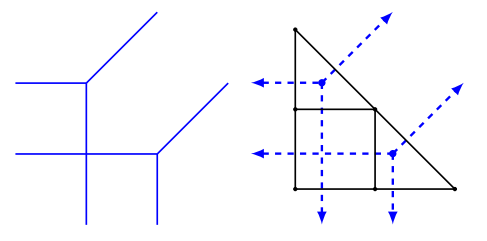
\includegraphics{tropical_curve.png}
		\caption{$1 \odot x_1^2 \oplus 1 \odot x_2^2 \oplus 2 \odot x_1x_2 \oplus 2 \odot x_1 \oplus 2 \odot x_2 \oplus 2.$ Слева: Тропическая кривая. Справа: двойственное разбиение многоугольника Ньютона и тропическая кривая.}
	\end{figure}

	\begin{figure}[h]
		\centering
		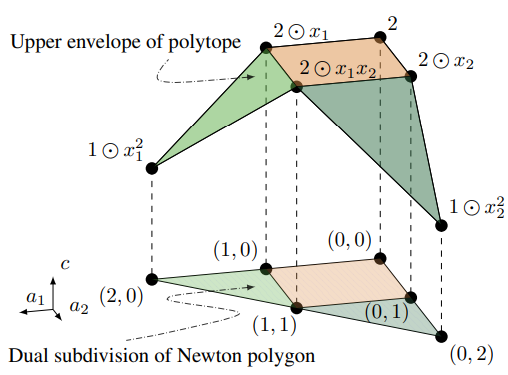
\includegraphics{dual_subdivision.png}
		\caption{$1 \odot x_1^2 \oplus 1 \odot x_2^2 \oplus 2 \odot x_1x_2 \oplus 2 \odot x_1 \oplus 2 \odot x_2 \oplus 2.$ Двоичное разбиение может быть получено проектированием краев верхних граней политопа.}
	\end{figure}

	Тропические гиперповерхности делят пространство $f$ на выпуклые ячейки, на каждой из которых $f$ линейна. Эти ячейки - выпуклые многогранники, т.е., определенные линейными неравенствами с целочисленными коэффициентами: ${x \in R^d : Ax \leq b}$ для $ A \in Z^{m \times d}$ и $b \in R^m$. Например, ячейка, где тропический моном $c_jx^{a_j}$ достигает максимума это $\{x \in R^d : c_j + a_j^Tx \geq c_i + a_i^Tx$ для всех $ i \neq j\}$. Тропические гиперповерхности многочленов от двух переменных (т.е. в $R^2$) называются \textit{тропическими кривыми}.
	
	Также, как и обычные многочлены, для каждого тропического многочлена есть соответствующий \textit{многоугольник Ньютона}.
	
	\begin{Definition}
		Многоугольником Ньютона тропического многочлена $f(x) = c_1x^{a_1} \oplus ... \oplus c_r x^{a_r}$ называют выпуклую оболочку $a_1, ..., a_r \in \mathbb{N}^d$, рассматриваемые как точки в $\mathbb{R}^d$,
		\begin{equation*}
			\Delta(f) := Conv\{a_i \in \mathbb{R}^d : c_i \neq - \infty, i=1,...,r\}.
		\end{equation*}
	\end{Definition}

	Тропический многочлен $f$ определяет двоичное разбиение $\Delta(f)$, построенное следующим образом. Во-первых, необходимо поднять каждое $a_i$ из $\mathbb{R}^d$ в $\mathbb{R}^{d+1}$, добавляя $c_i$ как последнюю координату. обозначим выпуклую оболочку поднятых $a_1,...,a_r$ как:
	
	\begin{equation*}
		\mathcal{P}(f) := Conv\{(a_i, c_i) \in \mathbb{R} \times \mathbb{R} : i = 1,...,r\}.
	\end{equation*}
	
	Далее пусть $UF(\mathcal{P}(f))$ обозначает коллекцию верхних граней $\mathcal{P}(f)$, а $\pi : \mathbb{R}^d \times \mathbb{R} \to \mathbb{R}^d$ - проекция, опускающая последнюю координату. Тогда двойственное разбиение, определяемое $f$, это:
	
	\begin{equation*}
		\delta(f) := \{\pi (p) \subset \mathbb{R}^d : p \in UF(\mathcal{P}(f))\}.
	\end{equation*}
	
	$\delta(f)$ формирует многогранный комплекс с помощью $\Delta(f)$. По (Maclagan \& Sturmfels, 2015, Proposition 3.1.6) тропическая гиперповерхность $\mathcal{T}(f)$ это $(d-1)$-скелет многогранного комплекса, двойственного к $\delta(f)$. Это означает, что каждая вершина $\delta(f)$ соответствует одной "ячейке" в $\mathbb{R}^d$, где функция $f$ линейна. Таким образом, количество вершин в $\mathcal{P}(f)$ является верхней границей для количества линейных областей $f$.
	
	Рисунок 1 показывает многоугольник Ньютона и двойственное разбиение тропического многочлена $f(x_1, x_2) = 1 \odot x_1^2 \oplus 1 \odot x_2^2 \oplus 2 \odot x_1x_2 \oplus 2 \odot x_1 \oplus 2 \odot x_2 \oplus 2.$. Рисунок 2 показывает, как мы можем найти двойственное разбиение для данного тропического многочлена, следую вышеупомянутым инструкциям; дано детально и пошагово в разделе C.1.
	
	Тропические многочлены и тропические рациональные функции это, очевидно, кусочно-линейные функции. По существе, тропическое рациональное отобращение это кусочно линейное отображение, с которым связано понятие \textit{линейной области}.
	
	\begin{Definition}
		Линейным регионом $F \in Rat(d, m)$ называют максимальное связаное подмножество области, на котором $F$ линейна. Количество линейных регионов $F$ обозначается как $\mathcal{N}(F)$
	\end{Definition}
	
	Заметим, что тропическое \textit{полиномиальное} отображение $F \in Pol(d, m)$ имеет выпуклые линейные регионы, но тропическое \textit{рациональное} отображение $F \in Rat(d, n)$ в общем случае имеет невыпуклые линейные регионы. В Главе 6.3 мы используем $\mathcal{N}(F)$ как меру сложности для $F \in Rat(d, n)$, задаваемой нейронной сетью.
	 
			
	\section{Нейронные сети}
	
	Хотя мы и ожидаем, что читатель знаком с нейронными сетями без обратной связи, тем не менее, в этой короткой главе мы определим их, в первую очередь чтобы зафиксировать обозначения и указать на допущения, которые мы сохраним в течение этой статьи. Мы ограничим наше внимание на полносвязных нейронных сетях без обратной связи.
	
	Рассматривая отвлеченно, нейронная сеть с L-слоями без обратной связи это отображение $v : R^d \to R^p$, заданное композицией функций
	\begin{equation*}
		v = \sigma^{(L)} \circ p^{(L)} \circ \sigma^{(L-1)} \circ p^{L-1} \circ ... \circ \sigma^{(1)} \circ p^{(1)}
	\end{equation*}
	
	\textit{Преактивационные} функции $p^{(1)},...,p^{(L)}$ это аффинные преобразования, которое будет определено, а \textit{активационные} функции $\sigma^{(1)},...,\sigma^{(L)}$ выбираются и фиксируются далее.
	
	Обозначим \textit{ширину}, т.е. количество узлов l-го слоя как $n_l$, l=1,...,L-1. Установим $n_0 := d$ и $n_L = p$, соответственно размеры входа и выхода сети. Выход l-го слоя будет обозначен как
	\begin{equation*}
		v^{(l)} := \sigma^{(l)} \circ p^{(l)} \circ \sigma^{(l-1)} \circ p^{(l-1)} \circ ... \circ \sigma{(1)} \circ p^{(1)},
	\end{equation*}
	
	т.е. это отображение $v^{(t)} : \mathbb{R}^d \to \mathbb{R}^{n_l}$. Для удобства положим $v^{(0)}(x) := x$.
	
	Аффинная функция $p^{(l)} : \mathbb{R}^{n_{l-1})} \to \mathbb{R}^l$ задается матрицей \textit{весов} $A^{(l)} \in Z^{n_l \times n_{l-1}}$ и вектором \textit{смещения} $b^{(l)} \in R^{n_l}$:
	\begin{equation*}
		p^{(l)}(v^{(l-1)}) := A^{(l)}v^{(l-1)} + b^{(l)}
	\end{equation*}
	
	Координаты $(i, j)$ матрицы $A^{(l)}$ будут обозначены как $a_{ij}^{(l)}$ и $i$-я координата $b^{(l)}$ как $b_{i}^{(l)}$. Вместе они формируют \textit{параметры} слоя $l$.
	
	Для векторного входа $x \in \mathbb{R}^{n_l}, \sigma^{(l)}(x)$ должна пониматься в покоординатном смысле; так, $\sigma : \mathbb{R}^{n_l} \to \mathbb{R}^{n_l}$. Мы принимаем, что последний выход нейронной сети $v(x)$ будет передан в \textit{оценочную функцию (score function)} $s : \mathbb{R}^p \to \mathbb{R}^m$, которая зависит от применения. Когда сеть используется в качестве классификатора из $m$ классов, $s$ может быть, например, soft-max или сигмоидальной функцией. Оценочная функция довольно часто рассматривается как последний слой нейронноей сети, но это делается просто из удобства, и мы не будем так делать. Мы примем следующие небольшие положения об архитектуре нейронной сети без обратной связи и объясним далее, почему они на самом деле небольшие:
	
	\begin{enumerate}[label=(\alph*)]
		\item веса матриц $A^{(1)},...,A^{(L)}$ целочисленые;
		\item вектора смещений $b^{(1)},...,b^{(L)}$ рациональные;
		\item функции активаций $\sigma^{(1)},...,\sigma^{(L)}$ принимают форму 
		\begin{equation*}
		\sigma^{(l)}(x) := max\{x,t^{(l)}\},
		\end{equation*}
		где $t^{(l)} \in (R \cup \{- \infty \})^{n_l}$ называется пороговым вектором.
	\end{enumerate}

	Отныне все нейронные сети в нашей дальнейшей дискуссии будут соответствовать пункати (a)-(c).
	
	(b) довольно общий, но потери всеобщности нет и в (a), т.е. в ограничении весов $A^{(1)},...,A^{(l)}$ от вещественных матриц до целых, так как:
	\begin{itemize}
		\item вещественные веса могут быть приближены довольно близко рациональными весами;
		\item затем можно «очистить знаменатели» в этих рациональных весах путем умножения их на наименьшее общее кратное их знаменателей для получения целых весов;
		\item держим в голове, что масштабирование всех весов и смещений одной и той же положительной константой не влияет на работу нейронной сети. 
	\end{itemize}

	Активационная функция в (c) включает как ReLU $(t^{(l)} = 0)$, так и идентичное отображение $(t^{(l)} = - \infty)$ как частные случаи. В случаях не с ReLU наш тропический каркас будет поддерживать кусочно-линейные активации, такие как leaky ReLU, абсолютное значение, и, с небольшим усилием, может быть расширен до max pooling, сетей maxout и т.п. Но он не поддерживает такие активации, как, например, гиперболический тангенс и сигмоиду.
	
	В данной работе мы  рассматриваем нейросети с ReLU как на простейшую и наиболее каноничную модель нейронной сети,  из которой могут быть выведены другие варианты, эффективные в конкретных задачах. Учитывая, что мы ищем общие теоретические идеи, а не специфичную практическую эффективность, имеет смысл ограничить себя до этого простейшего случая. Более того, нейросети с ReLU уже воплощают некоторые наиболее важные элементы (и загадки), распространенные в большом ряде нейронных сетей (например, универсальное приближение, экспоненциальная экспрессивность); они работают хорошо на практике и часто выбираются для сетей прямого распространения. Мы не одни ограничиваем дискуссию до нейросетей с ReLU  (Montufar et al., 2014; Aroraet al., 2018).

	\section{Тропическая геометрия нейронных сетей}
	
	В разделе 5 нейронные сети определяются с помощью тропической алгебры, что позволяет нам изучать их с помощью тропической алгебраической геометрии. Мы покажем, что граница принятий решений нейронной сети ~--- это подмножество тропической гиперповерхности, соответствующего тропического полинома(Раздел 6.1). Мы увидим, что в некотором смысле, зонотопы образуют геомтрические строительные блоки для нейронных сетей (Раздел 6.2). Затем мы докажем, что геометрия функции, представленной нейронной сетью, становится значиттельно более сложной с увеличением ее количества слоёв.
	\subsection{Границы решений нейронной сети}
	
	Мы будем использовать тропическую геометрию и идеи из Раздела 5 для изучения границ решений нейронных сетей, фокусируясь на случае классификации двух категорий для ясности. Как объяснено в Разделе 4, нейронная сеть $\nu : \mathbf{R}^d \rightarrow \mathbf{R}^p$ вместе с выбором функции оценки $s: \mathbf{R}^p \rightarrow \mathbf{R}$ дают нам классификатор. Если выходное значение $s(\nu(x))$ превышает некоторый порог принятия решений $c$, то нейронная сеть предсказывает, что $x$ относится к одной категории (например, $x$ ~--- изображение кота), а в противном случае $x$ относится к другой категории (например, $x$ ~--- изображение собаки). Таким образом входной пространство разделено на два непересекающихся подмножества \textit{границей принятия решений $B := \{x \in \mathbf{R}^d : \nu(x) = s^{-1}(c)\} $}. Связанные области со значением выше порога и связные области со значением ниже порога будем называть \textit{положительными} и \textit{отрицательными областями} соответственно.
	
	Предоставим оценки на количество положительных и отрицательных областей и покажем, что существует тропический многочлен, чья тропическая гиперповерхность содержит границу решений.
	\begin{Proposition}
		(Тропическая геометрия границы решений). Пусть $\nu : \mathbf{R}^d \rightarrow \mathbf{R}$  ~--- $L$-слойная нейронная сеть, удовлетворяющая предположению $(a)-(c)$ с $t^{(L)} = -\infty$. Пусть функция счета $s : \mathbf{R} \rightarrow \mathbf{R}$  является иньъективной с порогом принятия решений $c$ в его диапазоне. Если $\nu = f \oslash g$, где $f$ и $g$ ~--- тропические многочлены, тогда 
		\begin{enumerate}
			\item Его граница решений $B = \{x \in \mathbf{R}^d:\nu(x) = s^{-1}(c)\}$ делит $\mathbf{R}^d$ на не более чем $N(f)$ связных положительных областей и не более, чем $N(g)$ связных отрицательных областей;
			\item Его раница решений содержится в тропической гиперповерхности тропического многочлена $s^{-1}\odot g(x)\oplus f(x) = \max\{f(x),g(x)+s^{-1}(c)\}$, то есть 
				\[B 
				\subset T(s^{-1}(c)\odot g \oplus f)
				\]  
		\end{enumerate}
	
		Функция $s^{-1}(c) \odot g \oplus f$ не обязательно линейна на каждой положительной или отрицательной области и поэтому ее тропическая гиперповерхность $T(s^{-1}(c)\odot g \oplus f)$ может дальше делить положительные или отрицательные области, полученные из $B$ на несколько линейных областей. В общем случае $\subset$ нельзя заменить на $=$.
	\end{Proposition}

	\subsection{Зонотопы как геометрические строительные блоки нейронной сети}
	
	Из раздела 3, мы знаем, что число областей тропической гиперповерхности $T(f)$ делит пространство на равное число вершин в двойственном разбиении многоугольника Ньютона, связанного с тропическим многочленом $f$. Это позволяет нам ограничить количество линейных областей нейронной сети, ограничивая число вершин в двойственном разбиении многоугольника Ньютона. 
	
	Мы начнём изучение того, как геометрия меняется от одного слоя к следующему в нейронной сети, более точнее:
	
	\begin{Question}
		Как тропические гиперповерхности тропических многочленов в $(l + 1)$-ом слое нейронной сети связаны с ими в $l$-ом слое?
		содержимое...
	\end{Question}
	
	Рекуррентное соотношение (2) описывает, как тропические многочлены, встречающиеся в $(l + 1)$-ом слое получаются из многочленов в $l$-ом слое, а именно, через три операции: тропическая сумма, тропическую степень и тропическое умножение. Напомним, что тропическая гиперповерхность тропического многочлена ~--- двойственно разбиение многогранника Ньютона тропического многочлена, который задается проекцией верхних граней на многогранники, определяемые формулой (1). Отсюда вопрос сводится к тому, как эти три операции преобразуют многогранники, а это рассматривается в утверждениях 3.1 и 3.2. Мы следуем обозначениям из Утверждения 5.1 для следующего результата.
	
	\begin{Lemma}
		Пусть $f_i^{(l)},g_i^{(l)},h_i^{(l)}$ тропические многочлены, созданные $i$-ым узлом в $l$-ом слое нейронной сети, то есть они определяются как (2). Тогда $P(f_i^{(l)}, P(g_i^{(l)},P(h_i^{(l)}$, являющиеся подмножествами $\mathbf{R}^{d+1}$, задаются следующим образом:
		\begin{enumerate}
			\item $P(g_i^{(1) \text{ и } P(h_i^{(1)}}$ являются точками.
			\item $P(f_i^{(1)}$ ~--- отрезок.
			\item $P(g_i^{(1) \text{ и } P(h_i^{(1)}}$ ~--- зонотопы.
			\item Для $l \geq 1$,
			\[
				P(h_i^{(l)}) = Conv[P(g_i^{(l)}\odot t_i^{(l)}) \cup P(h_i^{(l)})]
			\]
			
			Если $t_i^{(l)} \in \mathbf{R}$, и $P(f_i^{(l)}) = P(h_i^{(l)})$, если $t_i^{(l)} = -\infty$
			\item Для $l \geq  1, P(g_i^{(l+1)})\text{ и } P(h_i^{(l+1)}) $ взвешены суммы Минковского, 
			\[
				P(g_i^{(l+1)}) = \sum\limits_{j=1}^{n_l} a_{ij}^-P(f_i^{(l)}) + \sum\limits_{j=1}^{n_l} a_{ij}^+P(g_i^{(l)}),
			\]
			\[
			P(h_i^{(l+1)}) = \sum\limits_{j=1}^{n_l} a_{ij}^+P(f_i^{(l)}) + \sum\limits_{j=1}^{n_l} a_{ij}^-P(g_i^{(l)})
			\]
			\[
				+\{b_ie\},
			\]
			
			Где $a_{ij}, b_i$ записаны в матрице весов $A^(l+1) \in \mathbf{Z}^{n_{l+1}\times n_l}$ и вектор смещения $b^(l+1) \in \mathbf{R}^{n_l+1} \text{ и } e:= (0, \dots,0,1)\in \mathbf{R}^{d+1}$.			
		\end{enumerate}
		\end{Lemma}
		Завершение леммы 6.2 состоит в том, что зонотопы являются строительными блоками в тропической геометрии нейронных сетей. Зонотопы широко изучены в выпуклой геометрии и, среди прочего, они тесно связаны с расположением гиперплоскостей. Лемма 6.2 связывает нейронные сети с этим обширным объёмом работы, но полный смысл этого еще предстоит изучить. В разделе С.2, кроме того, мы покажем, как можно построить эти многогранники для двуслойных нейронных сетей.
		
		\subsection{Геометрическая сложность глубоких нейронных сетей}
		
		Мы обращаемся к инструментам из раздела 3 для изучения сложности нейронной сети, показывая, что глубокая сеть более выразительна, чем неглубокая. Наша мера сложности является геометрической: мы будему следовать (Montufar et al., 2014;
		Raghu et al., 2017) и использовать количество линейных областей кусочно-линейной функции $\nu : \mathbf{R}^d \rightarrow \mathbf{R}^p$ для измерения сложности $\nu$.
		
		\begin{Theorem}
			Пусть $\nu : \mathbf{R}^d \rightarrow \mathbf{R}$ является $L$-слоем вещественной нейронной сетью с прямой связью, удовлетворяющей (a)-(c). Пусть $t^{(L)} = -\infty$ и $n_l \geq d$ для всех $l = 1,\dots,L-1$. Тогда $\nu = \nu^{(L)}$ имеет максимум
			\[
				\prod\limits_{l=1}^{L-1}\sum\limits_{i = 0}^{d} \begin{pmatrix}
				n_l\\
				i
				\end{pmatrix}
			\]
			линейных областей. В частности, если $d\leq n_1,\dots ,n_{L-1} \leq n$, то число линейных областей $\nu$ ограничено $O(n^{d(L-1)})$.
		\end{Theorem}
		
		\begin{Proof}
			Если $L = 2$, то это следует непосредственно из Леммы 6.2 и Следствия 3.4. Случай, когда $L \geq 3$ находится в разделе 7, в дополнении.
		\end{Proof}
	
	Как отмечалось в (Raghu et al., 2017), эта верхняя граница близко соответствует нижней границе $\Omega ((\frac{n}{d}^{(l-1)d})  n^d)$ в (Montufar et al., 2014, Corollary 5), когда $n_1 = \cdots = n_{L-1} = n \geq d$. отсюда мы предполагаем, что число линейных областей нейронной сети растёт полиномиально с шириной $n$ и экспоненциально с количеством слоёв $L$.
	
	\subsection{Заключение}
	
	Мы утверждаем, что прямые нейронные сети с выпрямленными узлами не что иное, как тропические рациональные карты. Чтобы понять их, нам зачастую нужно понимать соответствующую тропическую геометрию.
	
	В этой статье мы сделали первый шаг, чтобы предоставить подтверждение концепции: вопросы, касающиеся границ решений, линейных областей, как глубина влияет на выразительность и т.д. можно перевести на вопросы, касающиеся тропических гиперповерхностей, разбиений многоугольника Ньютона, многогранников, построенных из зонотопов и др.
	
	Как новая ветвь алгебраической геометрии, новшество тропической геометрии происходит из алгебры и геометрии и их взаимодействует друг с другом. Она связана множеством других областей математики. Среди прочих вещей, существует тропический аналог линейной алгебры и тропический аналог выпуклой геометрии. Мы затронули лишь небольшую часть этого богатого предмета. Мы надеемся, что дальнейшее исследование под тропическим углом поможет разгадать другие загадки глубоких нейронных сетей.
	
\end{document}